\documentclass{beamer}

\usetheme{Copenhagen}
\setbeamercolor{structure}{fg=red!75!black}
\setbeamertemplate{navigation symbols}{}
\setbeamertemplate{headline}{}
\usepackage{transparent}
\logo{\transparent{0.03}
\includegraphics[width=1.3\textwidth]{img/unimi_logo.pdf}}

\usepackage{settings-seminario}

\title{Automi 2-limited e linguaggi context-free}
\author{Alessandro Clerici Lorenzini}
\date{luglio 2023}
\institute{Seminario per l'esame di Teoria dei Linguaggi @ Unimi}

\begin{document}
\maketitle


\section{Introduzione}


\section{Automi \texorpdfstring{$2$}{2}-limited}
\begin{frame}{Automi $d$-limited}
	\begin{itemize}
		\item Hibbard (1967), caratterizzazione del determinismo nei linguaggi liberi dal contesto
		\item $d$-limited (\la d): restrizione di una macchina di Turing e al contempo generalizzazione degli automi \emph{two-way}:
		      \begin{itemize}
			      \item spazio di lavoro limitato alle celle contenenti l'input tramite \emph{end-marker}
			      \item scrittura su ciascuna cella solo durante le sue prime $d$ visite
		      \end{itemize}
		\item $M=(Q,\Sigma,\Gamma,\delta,q_0,F)$, $\Gamma$ partizionato in $\Sigma=\Gamma_0,\Gamma_1,\dots,\Gamma_d$
	\end{itemize}

	\vfill
	\begin{figure}
		\centering
		\begin{tikzpicture}[cell/.style={minimum height=1.5em,minimum width=1.5em,outer sep=0pt,rectangle,draw,node distance=0pt}]
	\node (lem) {\Large $\lem$};
	\node[cell] (0) [right=of lem]{$\sigma_0$};
	\node[cell] (1) [right=of 0] {$\sigma_1$};
	\node[cell] (2) [right=of 1] {$\sigma_2$};
	\node[cell] (3) [right=of 2] {$\sigma_3$};
	\node[cell, minimum width=2.5em] (worddots) [right=of 3] {$\dots$};
	\node[cell] (last) [right=of worddots] {$\sigma_n$};
	\node[node distance=0pt] (rem) [right=of last]{\Large $\rem$};
	\node[cell] (control) [below=0.75cm of 2,thick] {$q$};
	\draw[-latex,thick] (control) -- (2);
\end{tikzpicture}

	\end{figure}
\end{frame}

\begin{frame}{Automi $2$-limited: esempi}
	\only<1>{
		\framesubtitle{Linguaggi a blocchi}
		$K_n$ è il linguaggio delle stringhe in $\set{0,1}$ composte da blocchi di lunghezza $n$ tali che almeno $n$ blocchi sono uguali all'ultimo:
		\begin{align*}
			K_n := \{ & x_1x_2\cdots x_kx\mid k\geq0,x_1,\dots x_k,x\in\set{0,1}^n,                    \\
			          & \exists i_1<i_2<\dots<i_n\in\set{1,\dots,k},x_{i_1}=x_{i_2}=\dots=x_{i_n}=x \}
		\end{align*}
		Mostriamo un \la2 per $K_n$
	}
	\only<2>{
		\framesubtitle{Linguaggi di Dyck}
		Dato $k\in\N^+$
		\begin{itemize}
			\item $\Omega_k$ è l'alfabeto composto da $k$ tipi di parentesi ($2k$ simboli in tutto)
			\item $D_k$ è il linguaggio delle parentesi bilanciate su $\Omega_k$, detto linguaggio di Dyck.
		\end{itemize}
		\vspace{1cm}
		Mostriamo come un \la2 può riconoscere $D_k$
	}
\end{frame}

\begin{frame}{Potenza riconoscitiva: tutti i linguaggi context-free}
	\setbeamercovered{highly dynamic}
	\begin{theor}[di Chomsky-Schützenberger]
		Se $L$ è un linguaggio context-free su alfabeto $\Sigma$, esistono un naturale $k\in0$, un linguaggio regolare $R$ e un omomorfismo $h:\Omega_k\to\sigma\star$ tali che
		\begin{equation*}
			L=h(D_k\cap R)
		\end{equation*}
	\end{theor}
	\onslide<2>{
		\vfill
		Un \la2 può simulare il comportamento di una composizione di macchine:
		\begin{itemize}
			\item una macchina one-way che su input $w$ produce nondeterministicamente una stringa $z\in h^{-1}(w)$;
			\item il \la2 presentato precedentemente per $D_k$;
			\item un automa a stati finiti per $R$.
		\end{itemize}
	}
\end{frame}

\begin{frame}{Potenza e complessità: altre facce della medaglia}
	\begin{itemize}
		\item i \la2 riconoscono solo context-free? I.e., si possono convertire in PDA?
		\item qual è il rapporto di complessità tra le diverse descrizioni (PDA, \la2)?
		\item cosa succede nel caso deterministico?
	\end{itemize}
\end{frame}

\section{Da \texorpdfstring{$2$}{2}-limited a PDA}
\begin{frame}{Da \texorpdfstring{$2$}{2}-limited a PDA}
	\only<1>{
		\framesubtitle{Tabelle di transizione}
		\begin{columns}[t]
			\column{0.5\textwidth}
			\begin{figure}[h]
				\centering
				\begin{tikzpicture}
	\footnotesize
	\node[tapeseg] (w) {$w$};
	\draw	([xshift=-2cm]w.north) -- ([xshift=+2cm]w.north)
		([xshift=-2cm]w.south) -- ([xshift=+2cm]w.south);
	\node at ([yshift=-0.3cm, xshift=-2.3cm]w.south) (q) {$q$};
	\node (p) [below=.2 of q] {$p$};
	\draw	(q.east) -- ++(+2cm,-.12cm)
		-- ++(-.9cm,-.09cm) -- ++(+1.8cm,-.10cm)
		-- ++(-2.7cm,-.12cm) -- ++(+1.55cm,-.10cm)
		-- (p.east);
\end{tikzpicture}

				\caption{$(q,-1,p,-1)\in\tau_w$}
			\end{figure}
			\begin{figure}[h]
				\centering
				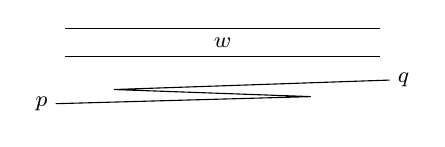
\begin{tikzpicture}[tapeseg/.style={minimum height=1.2em,minimum width=1.5em,outer sep=0pt,node distance=0pt}]
	\footnotesize
	\node[tapeseg] (w) {$w$};
	\draw	([xshift=-2cm]w.north) -- ([xshift=+2cm]w.north)
		([xshift=-2cm]w.south) -- ([xshift=+2cm]w.south);
	\node at ([yshift=-0.3cm, xshift=+2.3cm]w.south)	(q) {$q$};
	\node at ([yshift=-6mm, xshift=-2.3cm]w.south)		(p) {$p$};
	\draw	(q.west) -- ++(-3.5cm,-.12cm)
		-- ++(+2.5cm,-.09cm) -- (p.east);
\end{tikzpicture}

				\caption{$(q,+1,p,-1)\in\tau_w$}
			\end{figure}
			\column{0.5\textwidth}
			\begin{figure}[h]
				\centering
				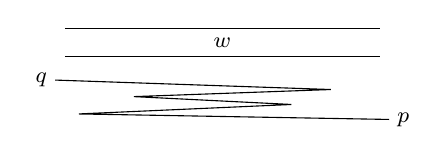
\begin{tikzpicture}[tapeseg/.style={minimum height=1.2em,minimum width=1.5em,outer sep=0pt,node distance=0pt}]
	\footnotesize
	\node[tapeseg] (w) {$w$};
	\draw	([xshift=-2cm]w.north) -- ([xshift=+2cm]w.north)
		([xshift=-2cm]w.south) -- ([xshift=+2cm]w.south);
	\node at ([yshift=-0.3cm, xshift=-2.3cm]w.south)	(q) {$q$};
	\node at ([yshift=-8mm, xshift=2.3cm]w.south)		(p) {$p$};
	\draw	(q.east) -- ++(+3.5cm,-.12cm)
		-- ++(-2.5cm,-.09cm) -- ++(+2cm,-.10cm)
		-- ++(-2.7cm,-.12cm) -- (p.west);
\end{tikzpicture}

				\caption{$(q,-1,p,+1)\in\tau_w$}
			\end{figure}
			\begin{figure}[h]
				\centering
				\begin{tikzpicture}
	\footnotesize
	\node[tapeseg] (w) {$w$};
	\draw	([xshift=-2cm]w.north) -- ([xshift=+2cm]w.north)
		([xshift=-2cm]w.south) -- ([xshift=+2cm]w.south);
	\node at ([yshift=-0.3cm, xshift=2.3cm]w.south) (q) {$q$};
	\node (p) [below=.1 of q] {$p$};
	\draw	(q.west) -- ++(-2cm,-.12cm)
		-- ++(+.9cm,-.09cm) -- ++(-1.8cm,-.10cm)
		-- (p.west);
\end{tikzpicture}

				\caption{$(q,+1,p,+1)\in\tau_w$}
			\end{figure}
		\end{columns}
		\vfill
		Composizione: $\tau_w\cdot\tau_z:=\tau_{wz}$
	}
	\only<2>{
		\framesubtitle{Tabelle di uscita}
		\begin{columns}[t]
			\column{0.5\textwidth}
			\begin{figure}[h]
				\centering
				\begin{tikzpicture}[tapeseg/.style={minimum height=1.1em,minimum width=1.5em,outer sep=0pt,node distance=0pt}]
	\footnotesize
	\node[tapeseg] (center) {};
	\node[tapeseg,node distance=.5] (w) [left=of center] {$w$};
	\node[tapeseg,node distance=.5] (z) [right=of center] {$z$};
	\draw	([xshift=-2cm]center.north) -- ([xshift=+2cm]center.north)
	([xshift=-2cm]center.south) -- ([xshift=+2cm]center.south)
	(center.north) -- (center.south);
	\node (q) at ([xshift=2mm,yshift=-3mm]center.south) {$q$};
	\node (p) at ([xshift=-2.2cm,yshift=-7mm]center.south) {$p$};
	\draw	(q.west) -- ++(-1cm,-.12cm)
	-- ++(+2.5cm,-.09cm) -- (p.east);
\end{tikzpicture}

				\caption{$(p,-1)\in\exitt(\tau_w,q,-1,\tau_z)$}
			\end{figure}
			\begin{figure}[h]
				\centering
				\begin{tikzpicture}[tapeseg/.style={minimum height=1.1em,minimum width=1.5em,outer sep=0pt,node distance=0pt}]
	\footnotesize
	\node[tapeseg] (center) {};
	\node[tapeseg,node distance=.5] (w) [left=of center] {$w$};
	\node[tapeseg,node distance=.5] (z) [right=of center] {$z$};
	\draw	([xshift=-2cm]center.north) -- ([xshift=+2cm]center.north)
	([xshift=-2cm]center.south) -- ([xshift=+2cm]center.south)
	(center.north) -- (center.south);
	\node (q) at ([xshift=-2mm,yshift=-3mm]center.south) {$q$};
	\node (p) at ([xshift=-2.2cm,yshift=-7mm]center.south) {$p$};
	\draw	(q.east) -- ++(1cm,-.12cm)
	-- ++(-2.5cm,-.09cm) -- ++(1cm,-.09cm)
	-- (p.east);
\end{tikzpicture}

				\caption{$(p,-1)\in\exitt(\tau_w,q,+1,\tau_z)$}
			\end{figure}
			\column{0.5\textwidth}
			\begin{figure}[h]
				\centering
				\begin{tikzpicture}
	\footnotesize
	\node[tapeseg] (center) {};
	\node[tapeseg,node distance=.5] (w) [left=of center] {$w$};
	\node[tapeseg,node distance=.5] (z) [right=of center] {$z$};
	\draw	([xshift=-2cm]center.north) -- ([xshift=+2cm]center.north)
	([xshift=-2cm]center.south) -- ([xshift=+2cm]center.south)
	(center.north) -- (center.south);
	\node (q) at ([xshift=2mm,yshift=-3mm]center.south) {$q$};
	\node (p) at ([xshift=2.2cm,yshift=-7mm]center.south) {$p$};
	\draw	(q.west) -- ++(-1cm,-.12cm)
	-- ++(+2.5cm,-.09cm) -- ++(-3cm,-.09cm)
	-- (p.west);
\end{tikzpicture}

				\caption{$(p,+1)\in\exitt(\tau_w,q,-1,\tau_z)$}
			\end{figure}
			\begin{figure}[h]
				\centering
				\begin{tikzpicture}
	\footnotesize
	\node[tapeseg] (center) {};
	\node[tapeseg,node distance=.5] (w) [left=of center] {$w$};
	\node[tapeseg,node distance=.5] (z) [right=of center] {$z$};
	\draw	([xshift=-2cm]center.north) -- ([xshift=+2cm]center.north)
	([xshift=-2cm]center.south) -- ([xshift=+2cm]center.south)
	(center.north) -- (center.south);
	\node (q) at ([xshift=-2mm,yshift=-3mm]center.south) {$q$};
	\node (p) at ([xshift=2.2cm,yshift=-7mm]center.south) {$p$};
	\draw	(q.east) -- ++(1.5cm,-.12cm)
	-- ++(-2.8cm,-.09cm) -- ++(1cm,-.09cm)
	-- ++(-1.3cm,-.09cm) -- (p.west);
\end{tikzpicture}

				\caption{$(p,+1)\in\exitt(\tau_w,q,+1,\tau_z)$}
			\end{figure}
		\end{columns}
	}
\end{frame}
\begin{frame}{PDA per $L\rem$}
	\only<1>{
		\framesubtitle{Definizioni}
		$L\in\mathrm{CFL}$

		$M=(Q,\Sigma,\Gamma,\delta,q_0,F)$ tale che $\genlang(M)=L$

		Costruiamo $M'=(Q',\Sigma,\Gamma',\delta',q_0',Z_0',F')$ tale che $\genlang(M')=L\rem$

		\begin{gather*}
			Q':=Q\cup Q\times\set{\tau_w\mid w\in\Sigma\star} \\
			\Gamma':=\Gamma\cup\set{\tau_w\mid w\in\Sigma\star}
		\end{gather*}

		\begin{itemize}
			\item Mantiene sulla pila lo stato del nastro di $M$ fino al simbolo letto, usando simboli per celle riscrivibili e tabelle per i segmenti congelati.
			\item In \emph{normal mode} legge il prossimo simbolo e carica sulla pila quanto scritto da $M$, in \emph{back mode} simula il comportamento di $M$ in una computazione nella parte del nastro già visitata, agendo per $\emptyword$-mosse sulla pila.
		\end{itemize}
	}
	\only<2>{
		\framesubtitle{Funzionamento}
		Mostriamo il funzionamento lavorando su un nastro d'esempio:
		\begin{figure}
			\centering
			\begin{tikzpicture}
	\footnotesize
	% \node[cell] (a) {$a$};
	\node[cell] (a) {\lower 1.5ex \hbox{$a$}};

	\node[cell] (b) [right=of a] {$b$};
	\node[cell,minimum width=40pt] (rd) [right=of b]{$\cdots$};
	\node[node distance=0pt] (rem) [right=of rd]{\Large $\rem$};

	\node[cell,minimum width=30pt] (f) [left=of a]{$F$};
	\node[cell] (y) [left=of f]{$Y$};
	\node[cell,minimum width=40pt] (ld) [left=of y]{$\cdots$};
	\node[node distance=0pt] (rem) [left=of ld]{\Large $\lem$};

	\node (p) [below=.35 cm of a] {$p$};
	\draw[-latex,shorten >=1pt] (p) -- (a);
\end{tikzpicture}
\qquad
\begin{tikzpicture}[cell/.append style={minimum width=1.7em}]
	\footnotesize
	\node[cell] (d) {\lower -1.6ex \hbox{\vdots}};
	\node[cell] (Y) [above=of d] {$Y$};
	\node[cell] (F) [above=of Y] {$\tau_F$};
\end{tikzpicture}

		\end{figure}
		Con $Y\in\Gamma_1$, $F\in\Gamma_2^+$, $a,b\in\Sigma=\Gamma_0$, $p\in Q$
	}
	\only<3>{
		\framesubtitle{Normal mode}
		In normal mode viene simulato direttamente il comportamento di $M$:
		\begin{figure}
			\centering
			\begin{tikzpicture}
	\footnotesize
	\node[cell] (a) {$a$};
	\node[cell] (b) [right=of a] {$b$};
	\node[cell,minimum width=40pt] (rd) [right=of b]{$\cdots$};
	\node[node distance=0pt] (rem) [right=of rd]{\Large $\rem$};
	\node[cell,minimum width=40pt] (F) [left=of a]{$F$};
	\node[cell] (Y) [left=of F]{$Y$};
	\node[cell,minimum width=30pt] (ld) [left=of Y]{$\cdots$};
	\node[node distance=0pt] (lem) [left=of ld]{\Large $\lem$};

	\draw[shorten >=3pt,shorten <=3pt] (a.north east) -- (a.south west);
	\node[tapeseg] (X) [above=of a] {$X$};

	\node (p) [below=.35 cm of a] {$p$};
	\node (q) [below=.35 of b] {$q$};
	\draw[-latex,shorten >=1pt] (p) -- (a);
	\draw[-latex,shorten >=1pt] (q) -- (b);
	\draw[->] (p.south) .. controls +(down:2.5mm) and +(down:2.5mm) .. (q.south);
\end{tikzpicture}
\qquad
\begin{tikzpicture}[cell/.append style={minimum width=1.7em}]
	\footnotesize
	\node[cell] (d) {\lower -1.6ex \hbox{\vdots}};
	\node[cell] (Y) [above=of d] {$Y$};
	\node[cell] (F) [above=of Y] {$\tau_F$};
	\node[cell] (X) [above=of F] {$X$};
	\draw[->,shorten >=1pt,shorten <=1pt] (F.west) ..  node[left] {push} controls +(left:2.5mm) and +(left:2.5mm) .. (X.west);
\end{tikzpicture}

		\end{figure}
		\begin{equation*}
			(q,X,+1)\in\delta(p,a)
		\end{equation*}
		\vspace{1mm}
		\begin{center}
			Stato: $p\to q$
		\end{center}
	}
	\only<4>{
		\framesubtitle{Back mode: 1 - entrata}
		In back mode lo stato è una coppia $(q,T)$ composta dallo stato simulato $q$ di $M$ e la tabella di transizione $T$ dell'ultimo segmento congelato (i.e. quello che termina con l'ultima cella letta).
		\begin{figure}
			\centering
			\begin{tikzpicture}
	\footnotesize
	\node[cell] (a) {$X$};
	\node[cell] (b) [right=of a] {$b$};
	\node[cell,minimum width=40pt] (rd) [right=of b]{$\cdots$};
	\node[node distance=0pt] (rem) [right=of rd]{\Large $\rem$};
	\node[cell,minimum width=40pt] (F) [left=of a]{$F$};
	\node[cell] (Y) [left=of F]{$Y$};
	\node[cell,minimum width=30pt] (ld) [left=of Y]{$\cdots$};
	\node[node distance=0pt] (lem) [left=of ld]{\Large $\lem$};

	\node[tapeseg] (Z) [above=of b] {$Z$};
	\draw [decorate,decoration={brace}] (Z.north west) -- (Z.north east) node[midway, above=3pt] {\SnowflakeChevron};
	\draw[shorten >=3pt,shorten <=3pt] (b.north east) -- (b.south west);

	\node (q) [below=.35 of b] {$q$};
	\node[outer sep=1pt] (r) [below=.35 cm of a] {$r$};
	\draw[-latex,shorten >=1pt] (q) -- (b);
	\draw[-latex,shorten >=1pt] (r) -- (a);
	\draw[->] (q.south) .. controls +(down:2.5mm) and +(down:2.5mm) .. (r.south);
\end{tikzpicture}
\qquad
\begin{tikzpicture}[cell/.append style={minimum width=1.7em}]
	\footnotesize
	\node[cell] (d) {\lower -1.6ex \hbox{\vdots}};
	\node[cell] (Y) [above=of d] {$Y$};
	\node[cell] (F) [above=of Y] {$\tau_F$};
	\node[cell] (X) [above=of F] {$X$};
\end{tikzpicture}

		\end{figure}
		\begin{equation*}
			(r,Z,-1)\in\delta(q,b)
		\end{equation*}
		\vspace{1mm}
		\begin{center}
			Stato: $q\to (r,\tau_Z)$ \\
			$T:=\tau_Z$
		\end{center}
	}
	\only<5>{
		\framesubtitle{Back mode: 2 - simbolo da riscrivere}
		\begin{figure}
			\centering
			\begin{tikzpicture}
	\footnotesize
	\node[cell] (X) {$X$};
	\draw[shorten >=3pt,shorten <=3pt] (X.north east) -- (X.south west);
	\node[tapeseg] (Zp) [above=of X] {$Z'$};

	\node[cell] (Z) [right=of X] {$Z$};
	\node[cell,minimum width=40pt] (rd) [right=of Z]{$\cdots$};
	\node[node distance=0pt] (rem) [right=of rd]{\Large $\rem$};

	\node[cell,minimum width=30pt] (F) [left=of X]{$F$};
	\node[cell] (y) [left=of F]{$Y$};
	\node[cell,minimum width=40pt] (ld) [left=of y]{$\cdots$};
	\node[node distance=0pt] (rem) [left=of ld]{\Large $\lem$};

	\node[outer sep=1pt] (r) [below=.35 cm of X] {$r$};
	\draw[-latex,shorten >=1pt] (r) -- (X);
	\node[tapeseg,node distance=1pt] (salign) [left=of X] {};
	\node[outer sep=1pt] (s) [below=.35 of salign] {$s$};
	\draw[-latex,shorten >=1pt] (s) -- (salign);
	\draw[->] (r.south) .. controls +(down:2.5mm) and +(down:2.5mm) .. (s.south);
\end{tikzpicture}
\qquad
\begin{tikzpicture}[cell/.append style={minimum width=1.7em}]
	\footnotesize
	\node[cell] (d) {\lower -1.6ex \hbox{\vdots}};
	\node[cell] (Y) [above=of d] {$Y$};
	\node[cell] (F) [above=of Y] {$\tau_F$};
	\node[cell] (X) [above=of F] {$X$};
	\node[node distance=2pt] (state) [below=of d] {$(r,\tau_Z)\to (s,\tau_{Z'}\cdot T)$};
	\node[node distance=0pt] (T) [below=of state] {$T:=\tau_{Z'}\cdot T=\tau_{Z'Z}$};
	\draw[->,shorten >=1pt,shorten <=1pt] (X.west) ..  node[left] {pop} controls +(left:2.5mm) and +(left:2.5mm) .. (F.west);
	\draw (X.north east) -- (X.south west);
\end{tikzpicture}

		\end{figure}
		\begin{equation*}
			(s,Z',-1)\in\delta(r,X)
		\end{equation*}
		\vspace{1mm}
		\begin{center}
			Stato: $(r,T)\to (s,\tau_{Z'}\cdot T)$ \\
			$T:=\tau_{Z'}\cdot T=\tau_{Z'Z}$
		\end{center}
	}
	\only<6>{
		\framesubtitle{Back mode: 3 - segmento congelato}
		\begin{figure}
			\centering
			\begin{tikzpicture}[cell/.append style={minimum width=1.7em}]
	\footnotesize
	\node[cell] (d) {\lower -1.6ex \hbox{\vdots}};
	\node[cell] (Y) [above=of d] {$Y$};
	\node[cell] (F) [above=of Y] {$\tau_F$};
	\draw[->,shorten >=1pt,shorten <=1pt] (F.west) ..  node[left] {pop} controls +(left:2.5mm) and +(left:2.5mm) .. (Y.west);
	\draw (F.north east) -- (F.south west);
\end{tikzpicture}
\qquad
\begin{tikzpicture}
	\footnotesize
	\node[cell] (a) {$Z'$};
	\node[cell] (b) [right=of a] {$Z$};
	\node[cell,minimum width=40pt] (rd) [right=of b]{$\cdots$};
	\node[node distance=0pt] (rem) [right=of rd]{\Large $\rem$};
	\node[cell,minimum width=40pt] (F) [left=of a]{$F$};
	\node[cell] (Y) [left=of F]{$Y$};
	\node[cell,minimum width=30pt] (ld) [left=of Y]{$\cdots$};
	\node[node distance=0pt] (lem) [left=of ld]{\Large $\lem$};

	\draw [decorate,decoration={brace,amplitude=3pt}] ([yshift=2mm] F.north west) -- ([yshift=2mm] b.east|-F.north west) node[midway, above=3pt] {\SnowflakeChevron};
	\node[tapeseg] (salign) [left=of a] {};
	\node[outer sep=1pt] (s) [below=.35 of salign] {$s$};
	\node[outer sep=1pt] (t) [below=.9 cm of Y] {$t$};
	\draw[-latex,shorten >=1pt] (s) -- (salign);
	\draw[-latex,shorten >=1pt] (t) -- ++(0,.6cm);

	\draw	(s.south) -- ++(-1cm,-.12cm)
		-- ++(2cm,-.09cm) -- ++(-1.5cm,-.10cm)
		-- ++(.9cm,-.12cm) -- (t.south);
\end{tikzpicture}

		\end{figure}
		\begin{equation*}
			(t,-1)\in\exitt(\tau_F,s,-1,T)
		\end{equation*}
		\vspace{1mm}
		\begin{center}
			Stato: $(s,T)\to (t,\tau_F\cdot T)$ \\
			$T:=\tau_F\cdot T=\tau_{FZ'Z}$
		\end{center}
	}
	\only<7>{
		\framesubtitle{Back mode: 4 - uscita}
		\begin{figure}
			\centering
			\begin{tikzpicture}[cell/.append style={minimum width=1.7em}]
	\footnotesize
	\node[cell] (d) {\lower -1.6ex \hbox{\vdots}};
	\node[cell] (Y) [above=of d] {$Y$};
	\node[tapeseg] (align) [below=of Y] {};
	\draw[->,shorten >=1pt,shorten <=1pt] (Y.west) ..  node[left] {pop} controls +(left:2.5mm) and +(left:2.5mm) .. (align.west);
	\draw (Y.north east) -- (Y.south west);
\end{tikzpicture}
\quad
\begin{tikzpicture}
	\footnotesize
	\node[cell] (a) {$Z'$};
	\node[cell] (b) [right=of a] {$Z$};
	\node[cell,minimum width=40pt] (rd) [right=of b]{$\cdots$};
	\node[node distance=0pt] (rem) [right=of rd]{\Large $\rem$};
	\node[cell,minimum width=40pt] (F) [left=of a]{$F$};
	\node[cell] (Y) [left=of F]{$Y$};
	\node[cell,minimum width=30pt] (ld) [left=of Y]{$\cdots$};
	\node[node distance=0pt] (lem) [left=of ld]{\Large $\lem$};

	\draw[shorten >=3pt,shorten <=3pt] (Y.north east) -- (Y.south west);
	\node[tapeseg] (Zpp) [above=of Y] {$Z''$};
	\draw [decorate,decoration={brace,amplitude=3pt}] (Zpp.north west) -- (b.east|-Zpp.north west) node[midway, above=3pt] {\SnowflakeChevron};

	\node[outer sep=1.5pt] (t) [below=.35 of Y] {$t$};
	\node[tapeseg] (ualign) [right=of Y] {};
	\node[tapeseg] (u) [below=.35 of ualign] {$u$};
	\draw[-latex,shorten >=1pt] (t) -- (Y);
	\draw[-latex,shorten >=1pt] (u) -- (ualign);
	\draw[->] (t.south) .. controls +(down:2.5mm) and +(down:2.5mm) .. (u.south);

	\node[tapeseg] (valign) [right=of b] {};
	\node[tapeseg] (v) [below=1 cm of valign] {$v$};
	\draw[-latex,shorten >=1pt] (v) -- ++(0,.6cm);
	\draw	(u.south) -- ++(1.3cm,-.12cm)
		-- ++(-1cm,-.09cm) -- ++(1.6cm,-.10cm)
		-- ++(-2.3cm,-.12cm) -- (v.south);
\end{tikzpicture}
\quad
\begin{tikzpicture}[cell/.append style={minimum width=1.7em}]
	\footnotesize
	\node[cell] (d) {\lower -1.6ex \hbox{\vdots}};
	\node[cell] (Y) [above=of d] {$Y$};
	\node[cell] (T) [above=of Y] {$T$};
	\draw[->,shorten >=1pt,shorten <=1pt] (Y.west) ..  node[left] {push} controls +(left:2.5mm) and +(left:2.5mm) .. (T.west);
\end{tikzpicture}

		\end{figure}
		\begin{equation*}
			(u,Z'',+1)\in\delta(t,Y)
		\end{equation*}
		\vspace{1mm}
		Sia $(v,d)\in\exitt(\tau_{Z''},s,+1,T)$
		\begin{itemize}
			\item se $d=-1$, si aggiorna $T$ e si procede come in precedenza
			\item se $d=+1$, si esce dalla back mode nello stato $v$, effettuando una push di $T$
		\end{itemize}
		Stessa procedura nel caso di mossa a destra da nastro congelato
	}
\end{frame}


\section{Altri aspetti}
\begin{frame}{Da PDA a \texorpdfstring{$2$}{2}-limited: complessità}
	\only<1>{
		\framesubtitle{Upper bound}
		Adattando da $L\rem$ a $L$ si ottiene il teorema fondamentale
		\begin{theor}
			Ogni \la2 con $n$ stati e un alfabeto di lavoro di $m$ simboli può essere simulato da un PDA con $2n(2^{4n^2}+1)+1)$ stati e un alfabeto per la pila di $m+2^{4n^2}$ simboli.
		\end{theor}
	}
	\only<2>{
		\framesubtitle{Lower bound}
		\begin{theor}
			Per ogni $n\in\N^+$, esiste un linguaggio riconosciuto da un \la2 con $n$ stati per il cui riconoscimento un PDA necessita di un numero esponenziale in $n$ di stati.
		\end{theor}
	}
	\only<3>{
		\framesubtitle{Caso deterministico}
		\begin{theor}
			Per ogni D\la2 $M$ con $n$ stati e un alfabeto di lavoro di $m$ simboli che accetta un linguaggio $L$ si può costruire:
			\begin{itemize}
				\item un DPDA che accetti $L\rem$ con $n((2n+1)^{2n}+1)+1$ stati e un alfabeto per la pila di $m+(2n+1)^{2n}$ simboli
				\item un PDA che accetti $L$ con $2n((2n+1)^{2n}+1)+1$ stati e un alfabeto per la pila di $m+(2n+1)^{2n}$ simboli
				\item un DPDA che accetti $L$ di dimensione al più doppiamente esponenziale rispetto alla dimensione di $M$
			\end{itemize}
		\end{theor}
	}
\end{frame}

\begin{frame}{Altri risultati}
	\begin{theor}
		\begin{itemize}
			\item Per ogni DPDA $M$ esiste un D\la2 equivalente la cui dimensione è polinomiale in quella di $M$
			\item Per ogni PDA $M$ esiste un \la2 equivalente la cui dimensione è polinomiale in quella di $M$
			\item La classe dei linguaggi accettati da D\la2 coincide con quella dei linguaggi context-free deterministici
		\end{itemize}
	\end{theor}
\end{frame}

\end{document}
